\documentclass[nobib]{tufte-handout}

\title{Föreläsning 4: Sammanfattning av alla räkneproblem, samt cykler $\cdot$ 1MA020}

\author[Vilhelm Agdur]{Vilhelm Agdur\thanks{\href{mailto:vilhelm.agdur@math.uu.se}{\nolinkurl{vilhelm.agdur@math.uu.se}}}}

\date{29 januari 2024}


%\geometry{showframe} % display margins for debugging page layout

\usepackage{graphicx} % allow embedded images
  \setkeys{Gin}{width=\linewidth,totalheight=\textheight,keepaspectratio}
  \graphicspath{{graphics/}} % set of paths to search for images
\usepackage{amsmath}  % extended mathematics
\usepackage{booktabs} % book-quality tables
\usepackage{units}    % non-stacked fractions and better unit spacing
\usepackage{multicol} % multiple column layout facilities
\usepackage{lipsum}   % filler text
\usepackage{fancyvrb} % extended verbatim environments
  \fvset{fontsize=\normalsize}% default font size for fancy-verbatim environments

\usepackage{color,soul} % Highlights for text


\include{mathcommands.extratex}

\begin{document}

\definecolor{darkgreen}{rgb}{0.0627, 0.4588, 0.1451}

\maketitle% this prints the handout title, author, and date

\begin{abstract}
\noindent
Vi blickar tillbaka på de olika räkneproblem vi har studerat i den första delen av kursen, och börjar skönja ett mönster. Vi skriver upp tabellen av problem vi studerat hittills, och fyller sedan i de återstående cellerna.

Till slut disktuerar vi en jobbigare variant av problemet med människor som sitter runt ett runt bord, och använder denna för att introducera konceptet av cykler i en permutation.
\end{abstract}

\section{Den tolvfaldiga vägen}

Vi har studerat ett antal olika räkneproblem hittills i denna kurs, från de relativt enkla -- antalet permutationer -- till de mer invecklade, som antalet surjektioner. Vi har ett antal gånger talat om ifall objekt skall vara särskiljbara eller osärskiljbara, och också ifall lådor får lov att vara tomma eller måste innehålla minst ett objekt.

När vi talade om kompositioner fördelade vi osärskiljbara objekt i särskiljbara lådor -- och studerade både fallet där lådor fick vara tomma, och när de inte fick det. För surjektioner fördelade vi särskiljbara objekt i särskiljbara lådor, och kravet var att varje låda får ett objekt.

Vi börjar ana ett mönster här i hur våra problem kan se ut. Vi kan ha
\begin{enumerate}
  \item Särskiljbara objekt och särskiljbara lådor
  \item Osärskiljbara objekt och särskiljbara lådor
  \item Särskiljbara objekt och osärskiljbara lådor
  \item Osärskiljbara objekt och osärskiljbara lådor
\end{enumerate}
och vi kan ha olika krav på hur objekten fördelas i lådorna
\begin{enumerate}
  \item Generell -- lådor får vara tomma och får innehålla hur många objekt som helst
  \item Surjektiv -- varje låda måste innehålla något objekt
  \item Injektiv -- ingen låda får innehålla mer än ett objekt
\end{enumerate}
så sammanfattningsvis har vi en tabell med tolv stycken tänkbara kombinatorikproblem. Det kommer visa sig att vi i själva verket redan studerat sju av dem.

Under föreläsning två pratade vi om fördelningar av osärskiljbara objekt mellan särskiljbara personer, och gav en formel för deras antal i Proposition 7, men vi gav aldrig ett kort namn åt detta problem. Låt oss kalla en sådan fördelning för en \emph{multi-delmängd} till mängden av personer.

En \emph{multi-mängd} är som en vanlig mängd, fast den får innehålla ett och samma objekt mer än en gång. Så vi betraktar alltså fördelningen av objekt mellan personer som en multi-delmängd genom att tänka att varje person är med i multidelmängden lika många gånger som antalet objekt den fick.

Så låt oss rita denna tabell -- problem vi redan studerat är i svart text, problem vi inte sett innan är i \textcolor{darkgreen}{grön text}. Låt $N$ vara en mängd av $n$ \emph{objekt}, och $X$ vara en mängd av $x$ \emph{lådor}. Vi ser fördelningarna av objekt i lådor som en funktion $f: N \to X$.

\begin{fullwidth}
  \begin{tabularx}{\linewidth}{l|ccc}
      & Generellt $f$ & Injektivt $f$ & Surjektivt $f$\\
      \midrule
    Bägge särskiljbara & \specialcell{Ord ur $X$ av längd $n$\\ $x^n$} & \specialcell{Permutation ur $X$ av längd $n$\\ $\frac{x!}{(x-n)!}$} & \specialcell{Surjektion från $N$ till $X$\\$x!\stirlingPart{n}{x}$} \\
    Osärskiljbara objekt & \specialcell{Multi-delmängd av $X$\\ av storlek $n$\\$\binom{n + x - 1}{n}$} & \specialcell{Delmängd av $X$ av storlek $n$\\$\binom{x}{n}$} & \specialcell{Kompositioner av $n$\\av längd $x$\\$\binom{n - 1}{n - x}$} \\
    Osärskiljbara lådor & \specialcell{\textcolor{darkgreen}{Mängdpartition av $N$}\\ \textcolor{darkgreen}{ i $\leq x$ delar} \\\textcolor{darkgreen}{$\sum_{k=1}^{x} \stirlingPart{n}{k}$}} & \specialcell{\textcolor{darkgreen}{Mängdpartition av $N$}\\ \textcolor{darkgreen}{i $\leq x$ delar av storlek $1$}\\\textcolor{darkgreen}{$1$ om $n \leq x$, $0$ annars}} & \specialcell{Mängdpartition av $N$\\i $x$ delar\\$\stirlingPart{n}{x}$} \\
    Bägge osärskiljbara & \specialcell{\textcolor{darkgreen}{Heltalspartition av $n$ i $\leq x$ delar}\\\textcolor{darkgreen}{$p_x(n + x)$}} & \specialcell{\textcolor{darkgreen}{Sätt att skriva $n$ som}\\\textcolor{darkgreen}{summan av $\leq x$ ettor}\\\textcolor{darkgreen}{$1$ om $n \leq x$, $0$ annars}} & \specialcell{\textcolor{darkgreen}{Heltalspartitioner av $n$}\\ \textcolor{darkgreen}{i $x$ delar} \\\textcolor{darkgreen}{$p_x(n)$}} 
  \end{tabularx}
\end{fullwidth}

Låt oss ge argument för varför varje av cellerna i denna tabell faktiskt är vad som påstås.

Raden med bägge särskiljbara är den enklaste att fundera på. Om vi tar ett generellt $f$ räknar vi \emph{alla} funktioner från $N$ till $X$, utan begränsningar och utan att bekymra oss om särskiljbarhet. Ett annat ord för ``funktion från $N$ till $X$'' kan vara ``ord ur $X$ av längd $n$'' ifall vi tänker oss $N = [n]$. Att kräva att funktionen är injektiv är samma sak som att kräva att ingen bokstav dyker upp två gånger i ordet, vilket ju var vår definition av en permutation. Om det enda vi kräver är att funktionen är surjektiv är så klart vad vi räknar just surjektioner.

I raden med osärskiljbara objekt så kan vi tänka oss objekten som bollar vi lägger i lådorna. Om vi kan acceptera varje fördelning av bollar -- lådor får vara tomma eller innehålla mer än en boll -- är ju detta precis vårt scenario med att fördela mynt bland personer, vilket vi just gett namnet multi-delmängder. 

Om varje låda bara får innehålla noll eller en boll, och vi inte kan se skillnad på bollarna, bestäms varje fördelning av bollar bara av vilka lådor som har en boll och vilka som inte har en -- alltså av en delmängd av lådorna, och delmängden måste ha samma storlek som antalet bollar. 

Kräver vi att varje låda måste få en boll är vi i fallet med kompositioner, som vi definierade kort i slutet av biten om multi-delmängder -- vi kan få en sådan genom att först ge varje person ett mynt och sedan fördela ut resten av mynten fritt, så vi härleder lätt den formeln ur formeln för multi-delmängder.

I raden med osärskiljbara lådor får vi i stället tänka oss att objekten är distinkta, men vi lägger dem i högar (och tillåter oss högst $x$ olika högar) istället för i lådor -- så vi kan inte se skillnad på olika högar annat än på deras innehåll. 

Om vi kräver att vår funktion är surjektiv, alltså att varje av våra $x$ högar måste innehålla ett objekt, så begränsar vi oss till att dela upp våra objekt i exakt $x$ högar, och det problemet har vi ju redan studerat: Det är alltså att vi gör en mängdpartition av objekten i $x$ delar. 

Om vi inte kräver att funktionen är surjektiv tillåter vi ``tomma högar'', vilka ju resulterar i att vi har en uppdelning i ett mindre antal faktiska högar. Så formeln är bara att vi summerar den tidigare formeln över varje möjligt antal högar.

Fallet med injektiva $f$ och osärskiljbara lådor är korkat. Vi vill alltså dela upp våra objekt i högst $x$ stycken högar, men kräver att varje hög har som mest ett objekt. Så om $n \leq x$ är detta möjligt -- varje objekt får sin egen hög -- annars är det omöjligt. Så det finns alltid noll eller ett sätt att göra detta på.

I sista raden, när både objekten och lådorna är osärskiljbara, får vi tänka oss att vi har identiska bollar som vi lägger i högar. Vi kan varken fråga ``vilka bollar ligger i den högen'' eller ``vilken av högarna är det där'', vi kan bara se hur många högar av varje storlek det finns. Så låt oss definiera det räkningsproblem detta motsvarar:

\begin{definition}
  En \emph{heltalspartition} av ett heltal $n$ i $k$ delar är ett sätt att skriva $n$ som summan av $k$ stycken heltal större än noll. Ordningen vi skriver heltalen i i summan spelar ingen roll. 
  
  Vi betecknar antalet heltalspartitioner av $n$ i $k$ delar med $p_k(n)$.
\end{definition}

Till skillnad från varje annat räkneproblem vi studerat hittills finns det ingen enkel formel för $p_k(n)$ i termer av $k$ och $n$. Men det betyder inte att vi inte kommer kunna säga intressanta kombinatoriska saker om heltalspartitioner.

\begin{example}
  Det finns fem heltalspartitioner av $8$ i $4$ delar. Dessa är:
  \begin{align*}
    5 + 1 + 1 + 1 &= 8\\
    4 + 2 + 1 + 1 &= 8\\
    3 + 3 + 1 + 1 &= 8\\
    3 + 2 + 2 + 1 &= 8\\
    2 + 2 + 2 + 1 &= 8
  \end{align*}
\end{example}

Så i sista raden, när vi kräver att funktionen är surjektiv, alltså att vi har exakt $x$ högar, ges antalet sådana funktioner av $p_x(n)$. Om vi inte kräver att funktionen är surjektiv så räknar vi istället alla heltalspartitioner av $n$ i högst $x$ delar. Antalet sådana ges av $p_x(n+x)$ -- tänk att vi ger en etta till varje av de $x$ lådorna, och sedan fördelar resten fritt, för att motivera formeln.

Slutligen är sista radens mellersta cell, när vi kräver att funktionen är injektiv, korkad av ungefär samma skäl som varför cellen ovanför var det. Vad vi kräver är alltså att ingen hög får ha mer än ett objekt -- så vi skall skriva $n$ som summan av högst $x$ stycken ettor! Om $n \leq x$ kan vi göra det på ett enda sätt -- vi skriver $n$ som summan av $n$ stycken ettor -- annars går det inte.

\section{Stirlingtalen av första sorten}

I förra föreläsningen introducerade vi Stirlingtalen av \emph{andra} sorten, vilket ju leder en till att fråga vad den första sorten är. Så låt oss introducera ett problem till vilket dem är lösningen:

\begin{definition}
  Antag att $n$ personer skall sitta runt $k$ stycken osärskiljbara runda bord, och varje bord måste ha minst en person som sitter vid det. Då ges antalet sätt att placera personerna runt borden av $\stirlingCycle{n}{k}$, \emph{Stirlings cykeltal}. Stirlings cykeltal kallas också för \emph{Stirlingtalen av första sorten}.
\end{definition}

Till skillnad från Stirlings partitionstal finns det inte någon enkel formel för cykeltalen. Vi kan däremot bevisa följande resultat:

\begin{theorem}
  Det gäller, för alla $n \geq 1$, att
  $$\sum_{k=1}^{n} \stirlingCycle{n}{k} = n!.$$

  \begin{proof}
    Vi bevisar detta genom att uppvisa en bijektion mellan mängden av permutationer av längd $n$ ur $[n]$, vilka vi vet att det finns $n!$ av, och samlingen av sätt att placera personer runt ett godtyckligt antal runda bord, vilka vi vet per definition räknas av $\sum_{k=1}^{n} \stirlingCycle{n}{k}$.

    \begin{marginfigure}\label{fig_cycles_of_permutation}
      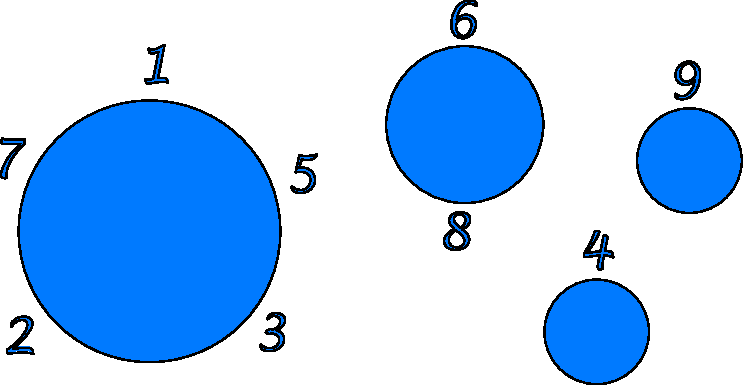
\includegraphics{graphics/cycles_of_permutation.pdf}
      \caption{Ett exempel på ett sätt placera nio personer vid runda bord. Den motsvarande permutationen till detta sätt att placera personer är $572438169$. Det vanliga sättet att skriva detta sätt att placera personer vid bord i text är $(15327)(4)(68)(9)$.}
    \end{marginfigure}

    Givet ett sätt att placera $n$ personer runt något antal runda bord kan vi definiera en permutation $\sigma$ genom att, på plats $i$ i permutationen, skriva den person som sitter till vänster om person $i$ runt deras bord. (En person som sitter ensam anser vi sitta till vänster om sig själv.) Detta kommer ge oss en permutation eftersom varje person bara har en person till höger om sig, så ingen person kommer dyka upp två gånger, och varje person har bara en person till vänster om sig, så $\sigma(i)$ är väldefinierat för varje $i$.

    Givet en permutation $\sigma$ kan vi placera ut personer runt runda bord som följer: Vi börjar med att ställa fram ett bord, och sätta person ett vid det bordet. Sedan sätter vi person $\sigma(1)$ till vänster om person ett, och person $\sigma(\sigma(1))$ till vänster om person $\sigma(1)$, och så vidare. Förr eller senare måste vi komma tillbaka till person $1$, eftersom det bara finns ändligt många personer. Om vi placerat alla personerna runt vårt första bord är vi klara.

    Om vi har några personer kvar att placera plockar vi fram ett till bord, och sätter den person med lägst nummer som inte redan har en sittplats vid det bordet -- säg att det är person $j$. Sedan upprepar vi processen från innan, och placerar person $\sigma(j)$ till vänster om henne, person $\sigma(\sigma(j))$ till vänster om person $\sigma(j)$, och så vidare. Återigen kommer vi förr eller senare komma tillbaka till person $k$, och ha gått full cirkel.

    Vi upprepar denna process med fler bord ända tills varje person har fått ett bord, och vi har fått oss ett sätt att placera $n$ personer runt något antal bord mellan $1$ och $n$.

    Det är någorlunda enkelt att se, efter att man funderat en stund, att vi alltid kommer komma tillbaka till samma permutation vi började med om vi först skapar en bordsplacering av permutationen, och sedan skapar en permutation av den bordsplaceringen. Alltså är detta en bijektion, och vi har bevisat vår formel.
  \end{proof}
\end{theorem}

\begin{remark}
  Vi har introducerat detta som ``personer runt runda bord'', men den vanliga matematiska terminologin runt detta är ``cykler i en permutation''. Hittills har vi bara sett permutationer som en lista av tal i någon ordning, där varje tal mellan $1$ och $n$ dyker upp exakt en gång, men detta är bara ett perspektiv på vad en permutation är.

  Perspektivet med cykler är ett minst lika vanligt perspektiv på permutationer, och framhäver andra saker man kan använda dem för. För att representera dessa i text skriver vi vanligen i formatet $(15327)(4)(68)(9)$, såsom i Figur \ref{fig_cycles_of_permutation}, i stället för att rita cirklar med tal runt dem.
\end{remark}

\section{Övningar}

\begin{xca}
  Ge ett kombinatoriskt bevis för följande rekursion för Stirlings cykeltal
  $$\stirlingCycle{n+1}{k} = \stirlingCycle{n}{k-1} + n\stirlingCycle{n}{k}.$$
\end{xca}

\begin{xca}
  I slutet av förra föreläsningen talade vi om \emph{derangemang} -- alltså permutationer $\sigma$ sådana att $\sigma(i) \neq i$ för alla $i$. Om vi i stället tänker på permutationer som sätt att placera personer runt runda bord, hur kan vi se på vår bordsplacering om vår permutation är ett derangemang?
\end{xca}

\begin{xca}
  Bevisa att\sidenote[][]{Här ber vi alltså inte specifikt om ett \emph{kombinatoriskt} bevis, även om beviset jag spontant kommer på är sådant. Om ni hittar ett induktionsbevis vore det också intressant.
  
  Ledtråd för det kombinatoriska beviset: Tänk att vi har ett speciellt objekt som är det $n+1$te, och det får hamna i sin speciella del. Så vi väljer hur stor den delen är och sedan fördelar vi ut resten av objekten.}
  $$\stirlingPart{n+1}{k+1} = \sum_{j=k}^{n} \binom{n}{j}\stirlingPart{j}{k}.$$
\end{xca}

\begin{xca}
  Skriv följande permutation av $[10]$ i cykelform
  $$8, 9, 4, 10, 5, 7, 3, 2, 6, 1.$$
\end{xca}

%\bibliography{references}
%\bibliographystyle{plainnat}

\end{document}
